\documentclass[12pt]{article}
\usepackage[left=2cm,right=2cm,top=2cm,bottom=2cm]{geometry}
\usepackage{wrapfig}
\usepackage{booktabs}
\usepackage{graphicx}
\usepackage{amssymb}
\usepackage{siunitx} % Required for alignment
\usepackage{subfigure}
\usepackage{multirow}
\usepackage{rotating}
\usepackage[T2A]{fontenc}
\usepackage[russian]{babel}
\usepackage{caption}
\usepackage{hyperref}
\usepackage{mathtools}
\usepackage{amsmath}
\usepackage{float}
\usepackage{mathrsfs}

\hypersetup{
    colorlinks=true,
    linkcolor=blue,
    urlcolor=magenta,
    citecolor=cyan,
    }
\graphicspath{{pictures/}}

\begin{document}
  \begin{titlepage}
      \begin{center}
          \vspace*{1cm}

          \Huge
          \textbf{ДИАМАГНЕТИЗМ И ПАРАМАГНЕТИЗМ}

          \vspace{1.5cm}

          \Large
          \textbf{Балдин Виктор Б01-303}

          \vfill

          Вопрос по выбору \\
          Устный экзамен по общей физике

          \vspace{0.8cm}

          
\includegraphics[width=0.4\textwidth]{university_logo.png}

          Физтех-школа радиотехники и компьютерных технологий\\
          Московский физико-технический институт\\
          Долгопрудный, 2024
      \end{center}
  \end{titlepage}

  \tableofcontents

  \section{Введение}
  Переходя к объяснению магнитных свойств материальных сред с атомистической точки зрения, заметим прежде всего, что в последовательно классической теории магнетизм должен отсутствовать. Бор в 1911 г. и независимо от него Ван-Лёвен в 1920 г., пользуясь методами классической статистики, строго доказали следующую теорему. В состоянии термодинамического равновесия система электрически заряженных частиц (электронов, атомных ядер и пр.), помещенная в постоянное магнитное поле, не могла бы обладать магнитным моментом, если бы она строго подчинялась законам классической физики. Такая система может быть намагничена только в неравновесном состоянии. Если она перейдет в равновесное состояние, то намагничивание исчезнет. Причина этого, грубо говоря, заключается в том, что постоянное магнитное поле, действуя на заряженную частицу с силой, перпендикулярной к скорости, не может изменить кинетическую энергию частицы. Для объяснения магнетизма вещества требуется привлечение квантовых представлений.

  Между тем парамагнетизм и диамагнетизм были объяснены, и притом довольно успешно, Ланжевеном (1872-1946) в 1905 г. без использования квантовых представлений. Причина этого заключается в том, что в классических теориях намагничивания молчаливо вводились представления сугубо квантового характера. Именно, предполагалось, что из электрически заряженных частиц можно построить устойчивые образования - атомы и молекулы. От последовательно классической теории надо требовать объяснения не только намагничивания, но и существования самих атомов, что удалось сделать только квантовой механике. Поскольку последняя в нашем курсе еще не излагалась, при объяснении намагничивания мы будем пользоваться полуклассическими представлениями. Несмотря на свою непоследовательность и недостаточность, полуклассическая теория позволяет в основном уяснить природу намагничивания.

  Начнем с краткого рассмотрения магнитных свойств атомов. Более подробно этот вопрос разобран в \cite{sivykhin5}. В простейшей боровской модели атома водорода электрон вращается вокруг ядра по окружности. Заряд электрона будем обозначать через $-\epsilon$. Вращающийся по окружности электрон в среднем возбуждает магнитное поле как ток $I=-e / T$, где $T=2 \pi r / v-$ период обращения электрона. Поэтому вращающемуся электрону присущ не только орбитальный момент импульса (или механический момент) $L=$ $=m r v$, но и магнитный момент $\mathfrak{M}=I S / c=-e r v /(2 c)$. Отношение этих величин называется гиромагнитным отношением и для нашей модели атома равно

  \begin{equation}
    \label{eq:intro}
    \Gamma=\frac{\mathfrak{M}}{L}=-\frac{e}{2 m c}
  \end{equation}


  Тот же результат справедлив для движений электрона по эллиптическим орбитам. Он верен и для многоэлектронных атомов, поскольку для всех электронов отношение $e / m$ одно и то же.

  Согласно теории Бора момент импульса атома квантуется, т.е. может принимать не непрерывный, а только дискретный ряд значений. Допустимыми являются значения $L=n \hbar$, где $n$ - целое число, которое может принимать значения $1,2,3, \ldots$, а $h=h /(2 \pi)=$ $=1,05 \cdot 10^{-27}$ эрг $+\mathrm{c}-$ постоянная Планка (1858-1947), деленная на $2 \pi$. (Эта величина также называется постоянной Планка и более удобна в теоретических вопросах.) Вместе с механическим моментом магнитный момент также квантуется в соответствии с формулой

  \begin{equation}
    \mathfrak{m}=-\frac{e \hbar}{2 m c} n
  \end{equation}


  Таким образом, наименьшее значение магнитного момента атома равно

  \begin{equation}
    \mathfrak{M}_{\mathrm{B}}=\frac{e \hbar}{2 m c}=9,28 \cdot 10^{-21} э \mathrm{pr} / \mathrm{Fc}
  \end{equation}

  Эта величина играет роль атома магнитного момента и называется магнетоном Бора.
  Квантовая механика оставила представление о движении электронов по классическим орбитам и уточнила правила квантования теории Бора. Вместо движения самих электронов квантовая механика ввела представление о движении некоторой величины, имеющей смысл плотности вероятности нахождения электрона в пространстве. Классическим, однако отнюдь не адекватным аналогом такого представления, может служить облако, в котором масса и соответствующий ей электрический заряд распределены в пространстве непрерывно с определенной плотностью. Существует дискретный ряд так называемых стационарных состояний, в которых эти величины не меняются во времени. К таким стационарным состояниям и относятся квантованные значения физических величин. Классическая формула (\ref{eq:intro}) для гиромагнитного отношения справедлива и в квантовой механике, как это непосредственно очевидно, если воспользоваться классическим аналогом квантовомеханического представления, о котором только что говорилось.

  В теории Бора электрон, обращающийся по орбите, становится эквивалентным току только после усреднения его положения вдоль орбиты. В квантовой механике, напротив, орбит нет и электрон в атоме, если его уподобить классической модели, вполне аналогичен току, непрерывно распределенному вокруг ядра атома.

  В боровской модели невозможны состояния, в которых орбитальные механический и магнитный моменты атомов равны нулю, так как в этом случае электрон должен был бы совершать радиальное движение, в котором он непременно столкнулся бы с ядром. Напротив, в квантовой механике возможны состояния со сферически симметричным распределением вероятности нахождения электрона вокруг ядра. В таких состояниях орбитальные механический и магнитный моменты электрона в атоме строго равны нулю.


  Наконец в квантовой механике формула $L=n \hbar$ определяет не полный момент количества движения электрона в атоме, а только проекцию этого вектора на избранное направление - направление магнитного поля, в которое помещен атом. Остальные две проекции не имеют определенных значений, что, конечно, невозможно представить в рамках классических моделей.

  4. Помимо орбитального электрон обладает еще собственным, или спиновым, моментом количества движения (короче, спином). В стационарных состояниях проекция спина на избранное направление может принимать только два значения: $+\hbar / 2$ и $-\hbar / 2$. Спину соответствует магнитный момент, проекция которого на избранное направление равна магнетону Бора. Таким образом, со спином электрона связано гиромагнитное отношение $\Gamma=-e /(m c)$, которое вдвое больше орбитального. Механический и магнитный моменты всякого атома, в том числе и многоэлектронного, векторно складываются из орбитальных и спиновых моментов. Могут существовать состояния, в которых механические и магнитные моменты скомпенсированы, т.е. полный момент атома равен нулю.

  \section{Термодинамика магнетиков}
  По аналогии с термодинамикой диэлектриков (см. \cite[\S31]{sivykhin3}) можно получить основные уравнения
  термодинамики магнетиков:
  \begin{align}
    \delta Q  &= dU - \frac{1}{4\pi}HdB,\\
    dU &= TdS + \frac{1}{4\pi}HdB,\\
    d\psi &= -SdT + \frac{1}{4\pi}HdB,\\ \label{eq:term4}
    d\Phi &= -SdT - \frac{1}{4\pi}BdH,\\
    dI &= TdS - \frac{1}{4\pi}BdH.
  \end{align}
  Для этого надо учесть, что элементарная внешняя работа равна $\delta A^{\text{внеш}} = (1/4\pi)HdB$.

  \section{Диамагнетизм}
  1. Диамагнетизм наблюдается у таких веществ, атомы которых в отсутствие магнитного поля не обладают магнитными моментами. Если нет магнитного поля, то на электрон в атоме действуют силы только со стороны атомного ядра и прочих электронов. В постоянном магнитном поле $\mathbf{B}$ к этим силам добавится сила $-(\epsilon / c)[\mathbf{v B}]$, где $\mathbf{v}-$ скорость электрона. Определим, как изменится движение атома в стационарном состоянии при наличии этой силы. С этой целью рассмотрим движение относительно системы отсчета, равномерно вращающейся
  вокруг направления магнитного поля с угловой скоростью $\boldsymbol{\Omega}$. Величину $\boldsymbol{\Omega}$ определим несколько ниже. Сейчас же будем предполагать, что она мала по сравнению с угловой скоростью $\boldsymbol{\text { собственного вращения }}$ электрона вокруг атомного ядра. При этом условии можно пренебречь всеми членами порядка $(\Omega / \omega)^2$, т. е. членами, квадратичными по $\Omega$. Во вращающейся системе отсчета к прежним силам добавятся две силы инерции: сила Кориолиса $2 m\left[\mathbf{v}_{\text {оти }} \boldsymbol{\Omega}\right]$ и центробежная сила. Центробежной силой мы пренебрежем, как величиной, пропорциональной $\Omega^2$, а в выражении кориолисовой силы относительную скорость электрона $\mathbf{v}_{\text {оти }}$ заменим абсолютной скоростью $\mathbf{v}=\mathbf{v}_{\text {оти }}+[\Omega \mathbf{r}]$. Такая замена также допустима, так как она меняет силу Кориолиса на величину, пропорциональную $\Omega^2$. В этом приближении кориолисова сила представится в виде $2 m[\mathbf{v} \boldsymbol{\Omega}]$. Подберем теперь величину $\boldsymbol{\Omega}$ так, чтобы выполнялось условие $2 m[\mathbf{v} \Omega]-(e / c)[\mathbf{v B}]=0$, т. е. положим

  \begin{equation}
  \label{eq:dia1}
  \boldsymbol{\Omega}=\frac{e}{2 m c} \mathbf{B}
  \end{equation}

  Тогда во вращающейся системе отсчета к прежним силам, действующим на электрон, не добавится никаких новых сил. Поэтому во вращающейся системе отсчета атом придет в то же стационарное состояние, в котором он находился в неподвижной системе в отсутствие магнитного поля. Если движение по-прежнему отнести к неподвижной системе отсчета, то получается следующий результат. При наличии внешнего постоянного магнитного поля внутреннее движение электронов атома не изменяется, но атом в целом получит дополнительное вращение с угловой скоростью (\ref{eq:dia1}). Этот результат называется теоремой Лармора (1857-1942), а величина $\Omega$ - ларморовской частотой.

  Остается проверить, выполняется ли условие $|\Omega| \ll|\omega|$, использованное при доказательстве. Очевидно, это условие можно записать так:

  \begin{equation}
  \label{eq:dia2}
  B \ll\left|\frac{2 m c \omega}{e}\right|
  \end{equation}


  Подставляя сюда численные значения $|e|=4,8 \cdot 10^{-10}$ СГСЭ-ед., $m=9,11 \cdot 10^{-28} \mathrm{r}, \omega \sim 10^{15} \mathrm{c}^{-1}$, получим $B \ll 10^8$ Гс. Рекордные магнитные поля, полученные до настоящего времени, не превосходят $10^7$ Гс. Поэтому условие (\ref{eq:dia2}) хорошо выполняется.

  2. Как видно из формулы (\ref{eq:dia1}), угловая скорость ларморовского вращения электронов совпадает по направлению с вектором B. Так как заряд электрона отрицательный, то магнитный момент, связанный с этим вращением, направлен против поля В. В результате создается намагничивание среды I, направленное также против поля В. Это и есть диамагнетизм.

  Рассчитаем теперь магнитную восприимчивость вещества. Электрон, вращающийся по окружности радиуса $r$ с ларморовской частотой $\boldsymbol{\Omega}$, обладает моментом импульса $m r^2 \boldsymbol{\Omega}$ и, следовательно, магнитным моментом $-e r^2 \Omega / 2 c=-e^2 r^2 \mathbf{H} /\left(4 m c^2\right)$. В последнем выражении вектор В заменен на $\mathbf{H}$, так как в диамагнетиках различие между этими векторами пренебрежимо мало. Если ось $Z$ перпендикулярна
  к плоскости круговой орбиты электрона, то $r^2=x^2+y^2$. Чтобы найти магнитный момент атома, надо просуммировать магнитные моменты всех его электронов. Электроны в атомах диамагнетика распределены сферически симметрично. В этом случае $\overline{x^2}=\overline{y^2}=\overline{z^2}=(1 / 3) \overline{R^2}$, где $R$ - расстояние электрона до ядра. Если атом содержит $Z$ электронов, то его средний магнитный момент в магнитном поле будет

  \begin{equation}
  \mathfrak{M}=-\frac{Z e^2}{4 m c^2}\left(\overline{x^2}+\overline{y^2}\right) H=-\frac{Z e^2}{6 m c^2} \overline{R^2} H,
  \end{equation}


  а вектор намагничивания среды

  \begin{equation}
  \label{eq:dia4}
  \mathbf{I}=-\frac{N Z e^2}{6 m c^2} \overline{R^2} \mathbf{H}
  \end{equation}


  где $N$ - число атомов в единице объема. Затем находим

  \begin{eqnarray}
  \varkappa=-\frac{N Z e^2}{6 m c^2} \overline{R^2}, \\
  \mu=1-\frac{4 \pi N Z e^2}{6 m c^2} \overline{R^2}
  \end{eqnarray}

  Энергия теплового движения слишком мала, чтобы изменить внутреннее (квантованное) состояние атома. Поэтому для диамагнетиков величины $ж$ и $\mu$ не должны зависеть от температуры. Этот вывод теории находится в согласии с опытом.

  Чтобы подтвердить, что теория находится на верном пути, оценим размеры атома, пользуясь значениями восприимчивости $\%$. Величина $\overline{R^2}$ должна вычисляться с помощью квантовой механики.

  Однако и без вычислений ясно, что квадратный корень из нее по порядку величины определяет размеры атома. Благородные газы, ввиду сферической симметрии электронных оболочек их атомов, диамагнитны. Диамагнитные свойства удобно характеризовать магнитной восприимчивостью па моль вещества $\chi_A$. Она связана с $\chi$ соотношением $\varkappa_A=V \varkappa$, где $V$ - объем одного моля. Величину $\varkappa_A$ можно вычислять по формуле (\ref{eq:dia4}), если под $N$ понимать число Авогадро (1776-1856). В случае гелия опыт дает $\varkappa_A=-2,2 \cdot 10^{-6}$; в случае аргона $\varkappa_A=$ $=-2,5 \cdot 10^{-4}$. Для гелия $Z=2$, для аргона $Z=18$. Подставляя
  эти данные в формулу (\ref{eq:dia4}), получим: Не, $\sqrt{R^2}=0,63 \cdot 10^{-8}$ см; Ar , $\sqrt{\overline{R^2}}=0,67 \cdot 10^{-8} \mathrm{cм}$. Эти результаты удовлетворительно согласуются с размерами атомов, найденными другими способами.

  3. Необходимо еще выяснить, какие силы сообщают атому ларморовское вращение. Этого не могут сделать магнитные силы, так как они перпендикулярны к скорости электрона и работы не производят. А с ларморовским вращением связана дополнительная кинетическая энергия атома. Магнитные силы могут только поддерживать, но не создавать ларморовское вращение. Последнее возникает во время включения магнитного поля. Переменное магнитное поле возбуждает вихревое электрическое поле. Оно-то и сообщает атому ларморовское
  вращение. Для пояснения допустим, что электрон вращается по окружности радиуса $r$, плоскость которой перпендикулярна к (однородному) магнитному полю В. Пусть магнитное поле включается адиабатически, т.е. настолько медленно, что за время одного оборота электрона по окружности поле почти остается постоянным. Ввиду симметрии вихревое электрическое поле $\mathbf{E}$ будет направлено по касательной к окружности. На основании закона электромагнитной индукции $2 \pi r E=$ $=-(1 / c) d \Phi / d t$, где $\Phi-$ магнитный поток, пронизывающий площадь, ограниченную той же окружностью. Отсюда и найдется поле Е. Момент сил, действующих на электрон, $M=-r e E=(e / 2 \pi c) d \Phi / d t$. На основании уравнения моментов

  \begin{equation}
  m r^2 \frac{d \Omega}{d t}=M=\frac{e}{2 \pi c} \frac{d \Phi}{d t}
  \end{equation}

  В начальный момент $B=\Omega=0$. Поэтому, интегрируя предыдущее уравнение, получим

  \begin{equation}
  m r^2 \Omega=\frac{e}{2 \pi c} \Phi
  \end{equation}

  откуда $\Omega=e B /(2 m c)$. Если изменение магнитного поля прекратится, то прекратится и дальнейшее изменение угловой скорости вращения атома. Последний будет продолжать вращаться с постоянной угловой скоростью, определяемой формулой Лармора (\ref{eq:dia1}).

  Из изложенного видно, что ларморовское вращение есть одно из проявлений электромагнитной индукции. То обстоятельство, что электромагнитная индукция должна приводить именно к диамагнетизму; а не к парамагнетизму, проще всего понять, руководствуясь принципом Ленца. Действительно, в соответствии с этим принципом магнитное поле $\mathbf{B}_{\text {мид }}$, возбуждаемое ларморовским вращением электронов, должно иметь такое направление, чтобы препятствовать всяким изменениям внешнего приложенного поля $\mathbf{B}$. Поэтому поле $\mathbf{B}_{\text {нис }}$ а с ним и вектор намагничивания среды I должны иметь направление, противоположное направлению внешнего поля В. Явление электромагнитной индукции имеет место во всех средах. Поэтому и обусловленный им диамагнетизм есть универсальное явление, которое должно проявляться во всех средах. Однако в тех случаях, когда атомы обладают собственными магнитными моментами, диамагнитный эффект перекрывается значительно более сильным парамагнитным эффектом.

  \section{Парамагнетизм}
  1. Парамагнетизм наблюдается у тех веществ, атомы которых обладают магнитными моментами уже в отсутствие внешнего магнитного поля. Пока нет магнитного поля, атомы совершают беспорядочное тепловое движение, а их магнитные моменты ориентированы в пространстве также беспорядочно. В этом случае тело не намагничено. В магнитном поле магнитные моменты атомов ориентируются преимущественно в направлении поля. Появляется намагничивание и обусловленный им парамагнетизм.

  Излагаемая ниже теория парамагнетизма относится к парамагнитным газам, взаимодействие между атомами которых слабое. Качественно результаты этой теории применимы также к твердым и жидким парамагнетикам, электронные оболочки атомов или ионов которых могут более или менее свободно вращаться вокруг атомных ядер. Это имеет место, например, тогда, когда электронные оболочки обладают сферической симметрией. Таковы электронные оболочки атомов благородных газов или ионов с таким же числом электронов, как у благородных газов.

  2. Поместим изолированный атом в постоянное магнитное поле В. Отвлечемся от наличия спинов, предполагая, что все спины электронной оболочки скомпенсированы. Пусть $\mathbf{v}$ - скорость какого-либо электрона атома до внесения в магнитное поле. Тогда, согласно теореме Лармора, в магнитном поле скорость того же электрона будет $\mathbf{v}+[\Omega \mathbf{r}]$, а его кинетическая энергия $(1 / 2) m(\mathbf{v}+[\boldsymbol{\Omega r}])^2$, где $\boldsymbol{\Omega}-$ ларморовская частота. Если пренебречь квадратами величины $\Omega$, то для приращения кинетической энергии электрона можно написать $m(\mathrm{v}[\Omega \mathrm{r}])$ или $m([\mathrm{rv}] \Omega)$. Просуммировав по всем электронам оболочки, находим приращение $\mathscr{\ell}$ кинетической энергии атома в магнитном поле: $\mathcal{C}=(\mathbf{L} \boldsymbol{\Omega})$, где $\mathbf{L}$ - момент импульса электронной оболочки. C помощью формул (\ref{eq:intro}) и (\ref{eq:dia1}) это выражение приводится к виду

  \begin{equation}
  \label{eq:12}
  \mathscr{\varepsilon}=-(\mathfrak{m} \mathbf{B}) .
  \end{equation}

  Такое же изменение энергии (но уже потенциальной) мы получили бы для магнитного диполя с магнитным моментом $\mathfrak{M}$ при внесении его в магнитное поле. Этого и следовало ожидать, так как, согласно теореме Ампера, во внешнем магнитном поле элементарный виток с током (например, вращающийся по орбите электрон) испытывает те же силы, что и магнитный диполь. Поэтому формула (\ref{eq:12}) для приращения энергии справедлива и в том случае, когда магнитный момент $\mathfrak{n}$ обусловлен спинами, а не орбитальным движением электронов. Вообще, формула (\ref{eq:12}) верна независимо от происхождения магнитного момента атома $\mathfrak{N}$, как это можно подтвердить независимым расчетом (см. п. 8).

  3. На основании изложенного ясно, что классическая теория парамагнетизма газов по существу не должна отличаться от соответствующей теории Дебая поляризации газообразных диэлектриков с полярными молекулами, которая была изложена в § 36. Теория парамагнетизма была создана Ланжевеном раньше теории диэлектриков Дебая. Последняя просто копирует теорию Ланжевена. Как видно из формулы (\ref{eq:12}), энергия атома больше, если его магнитный момент ориентирован против магнитного поля, и меньше, если он ориентирован по полю. Поэтому в состоянии статистического равновесия больше магнитных моментов будет ориентировано по полю, чем в противоположном направлении, т.е. будет наблюдаться парамагнетизм. Если выполнено условие

  \begin{equation}
  \label{eq:13}
  \frac{\mathfrak{M} B}{k T} \ll 1
  \end{equation}

  то, по аналогии с формулой (36.5), в классической теории можно написать

  \begin{equation}
  \label{eq:classic}
  \mathbf{I}=\frac{n \mathfrak{M}^2}{3 k T} \mathbf{B}
  \end{equation}

  Отсюда, используя соотношения $\mathbf{I}=\varkappa \mathbf{H}, \mathbf{B}=(1+4 \pi \varkappa) \mathbf{H}$, получим

  \begin{equation}
  \frac{\varkappa}{1+4 \pi \varkappa}=\frac{n \mathfrak{N}^2}{3 k T}
  \end{equation}


  Этой формулой и определяется магнитная восприимчивость парамагнетика. Впрочем, магнитная восприимчивость неферромагнитных тел настолько мала, что в предыдущей формуле, как это обычно делается, величиной $4 \pi \varkappa$ можно пренебречь по сравнению с единицей. Тогда

  \begin{equation}
  \label{eq:16}
  \varkappa=\frac{n \mathfrak{M}^2}{3 k T}
  \end{equation}

  4. Обобщим теперь формулы (\ref{eq:classic}) и (\ref{eq:16}) на случай сильных магнитных полей или низких температур, когда условие (\ref{eq:13}) не соблюдается. Это было сделано также Ланжевеном. Однако в классической теории Ланжевена не учитывается квантование магнитных моментов атомов, что существенно в области низких температур. Для учета квантования надо считать магнитный момент атома $\mathfrak{M}$ кратным магнетону Бора $\mathfrak{M}_{\mathrm{B}}$ и принять во внимание все ориентации его, допускаемые правилами квантования. Примем, что магнитный момент атома $\mathfrak{\Omega}$ спиновый и равен одному магнетону Бора. Такое предположение не затрагивает ничего существенного, обусловленного квантованием, но сильно упрощает расчет, так как в этом случае в магнитном поле возможны только две ориентации атома: параллельная и антипараллельная. В параллельной ориентации проекция магнитного момента на направление магнитного поля равна $+\mathfrak{M}_{\mathrm{B}}$, а антипараллельной $-\mathfrak{M}_{\mathrm{B}}$. (В дальнейшем значок В будем опускать.) Этим ориентациям соответствуют энергии $-\mathfrak{M} B$ и $+\mathfrak{M} B$. Согласно распределению Больцмана числа атомов (в единице объема) с параллельной и антипараллельной
  ориентациями будут равны соответственно

  \begin{equation}
  n_1=C e^x, \quad n_2=C e^{-x}
  \end{equation}

  где введено обозначение

  \begin{equation}
  x=\frac{\mathfrak{W} B}{k T}
  \end{equation}

  Нормировочная постоянная $C$ определится из условия $n_1+n_2=n$, где $n$ - полное число атомов в единице объема. Это дает $C\left(e^x+e^{-x}\right)=n$.
  ${ }^1$ Было бы непоследовательно учитывать различие между В и H и пренебрегать, как мы всюду делали в этом параграфе, различием между средним макроскопическим полем $\mathbf{B}$ и полем $\mathbf{B}^{\prime}$, действующим на атом парамагнетика, между квадратом среднего поля В и средним квадратом микроскопического поля и т. п. Все эти различия одного и того же порядка.
  Для намагничивания получаем $I=\left(n_1-n_2\right)\mathfrak{M}$, откуда

  \begin{equation}
  \label{eq:quantum}
  I=n \mathfrak{N} \frac{e^x-e^{-x}}{e^x+e^{-x}}=n \mathfrak{N} \text { th } x
  \end{equation}

  5. Прежде чем исследовать полученную формулу, заметим, что в случае, когда магнитный момент атома больше одного магнетона Бора, расчет проводится по той же схеме. Увеличивается только число возможных ориентаций и значения проекций магнитных моментов атомов на направление магнитного поля. Во всех случаях результат записывается в виде

  \begin{equation}
  I=n \mathfrak{M} L(x)
  \end{equation}

  где $L(x)$ называется функцией Ланжевена. В разобранном нами случае функция Ланжевена равна th $x$ и обозначается через $L_{1 / 2}(x)$, поскольку механический момент атома (в единицах $\hbar$ ) равен $1 / 2$. В других случаях вид функции $L(x)$ изменяется, но ее общий характер сохраняется. В классическом пределе, когда квантования нет, т. е. допустимы все ориентации магнитных моментов, функцию Ланжевена обозначают через $L_{\infty}(x)$. Она равна

  \begin{equation}
  \label{eq:lang}
  L_{\infty}(x)=\operatorname{cth} x-\frac{1}{x}
  \end{equation}

  (см. задачу к этому параграфу). Этот результат был получен самим Ланжевеном.
  6. Графики функций Ланжевена $L_{1 / 2}(x)$ и $L_{\infty}(x)$ приведены на рис. \ref{fig:175}. При малых $x$

  \begin{equation}
  L_{1 / 2}(x)=x-\frac{1}{3} x^3+\ldots, \quad L_{\infty}(x)=\frac{1}{3} x+\ldots
  \end{equation}

  В соответствии с этим в слабых полях ($x \ll 1$) I зависит от $\mathbf{B}$ линейно. По формуле \ref{eq:quantum} получается

  \begin{equation}
  \mathbf{I}=\frac{n \mathfrak{M}^2}{k T} \mathbf{B}
  \end{equation}

  а по формуле $(\ref{eq:lang})$ - классический результат $(\ref{eq:classic})$, т. е. величина втрое меньшая. Магнитные моменты $\mathfrak{N}$ определяются внутренним строением атома. Тепловое движение недостаточно интенсивно, чтобы изменить их. Поэтому, как видно из формулы (\ref{eq:12}0) или (\ref{eq:classic}), магнитная восприимчивость парамагнитных газов должна меняться обратно пропорционально абсолютной температуре $T$. Такая закономерность была обнаружена экспериментально II. Кюри еще до разработки соответствующей теории и носит название закона Кюри. Закон Кюри хорошо согласуется с опытом для газообразных парамагнетиков, а также для ряда твердых парамагнетиков (например, солей редких земель). С другой стороны, для многих жидких и твердых парамагнетиков изложенная элементарная теория недостаточна, поскольку она допускает свободное вращение электронных оболочек атомов вокруг направления магнитного поля. Впрочем, и в тех случаях, когда это
  допущение справедливо, в сильных полях ( $x \gg 1$ ) и при очень низких температурах (порядка нескольких Кельвинов) должны наблюдаться отклонения не только от закона Кюри, но и от самой пропорциональности между величинами I и $B$.

  \begin{figure}[H]
    \centering
    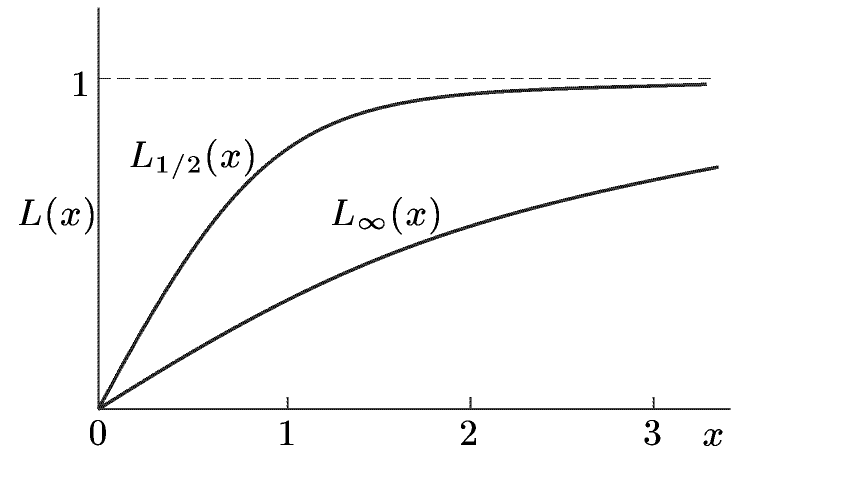
\includegraphics[width=0.6\textwidth]{graph.png}
    \caption{График $L(x)$}
    \label{fig:175}
  \end{figure}

  7. В сильных полях ( $x \gg 1$ ) обе функции $L_{1 / 2}(x)$ и $L_{\infty}(x)$ асимптотически стремятся к единиц. Этому соответствует насыщение намагничивания $I=n \mathfrak{N}$, когда все магнитные моменты устанавливаются параллельно магнитному полю. Однако классическая функция $L_{\infty}(x)$, как и следовало ожидать, не удовлетворяет тепловой теореме Нернста (1864-1941) (см. \cite{sivykhin2}), тогда как функция $L_{1 / 2}(x)$ согласуется с ней. В самом деле, в отсутствие квантования справедлива классическая теорема о равномерном распределении кинетической энергии по степеням свободы. Согласно этой теореме вращательные степени свободы атома должны быть возбуждены - на каждую из них придется кинетическая энергия $(1 / 2) k T$ и теплоемкость $(1 / 2) k$, не зависящая от температуры. При абсолютном нуле получилось бы конечное значение теплоемкости, что противоречит теореме Нернста. Другое противоречие с теоремой Нернста заключается в следующем. Из формул (73.3) и (73.4) следует

  \begin{equation}
  \left(\frac{\partial S}{\partial B}\right)_T=-\frac{1}{4 \pi}\left(\frac{\partial H}{\partial T}\right)_B, \quad\left(\frac{\partial S}{\partial H}\right)_T=\frac{1}{4 \pi}\left(\frac{\partial B}{\partial T}\right)_H
  \end{equation}

  Согласно теореме Нернста все процессы при абсолютном нуле температур не сопровождаются изменениями энтропии. Поэтому левые, а с ними и правые части полученных соотношений при $T=0$ должны обращаться в нуль:

  \begin{equation}
  \left(\frac{\partial H}{\partial T}\right)_B=\left(\frac{\partial B}{\partial T}\right)_H=0 .
  \end{equation}

  Если воспользоваться формулой $\mathbf{B}=\mathbf{H}+4 \pi \mathbf{I}$, то полученные результаты можно записать в виде

  \begin{equation}
  \left(\frac{\partial I}{\partial T}\right)_B=\left(\frac{\partial I}{\partial T}\right)_H=0
  \end{equation}

  Но классическая формула (\ref{eq:lang}) не согласуется с этими соотношениями. Действительно, при $x \gg 1$ справедлива асимптотика $L_{\infty}(x)=1-$ $-1 / x$ и, следовательно,

  \begin{equation}
  I=n \mathfrak{M}\left(1-\frac{1}{x}\right)=n \mathfrak{M}-\frac{n k T}{B}
  \end{equation}

  Из нее следует $(\partial I / \partial T)_B=n k / B$, т. е. при абсолютном нуле производная $(\partial I / \partial T)_B$ не обращается в нуль. Но если взять формулу (\ref{eq:quantum}), то можно воспользоваться асимптотикой $L_{1 / 2}(x)=1-2 e^{-2 x}$, и, следовательно, $I=n \mathfrak{M}\left(1-2 e^{-2 x}\right)$. Отсюда видно, что при $x \rightarrow \infty$ $I$ стремится к постоянному значению $n\mathfrak{M}$ (насыщение), а производная $\partial I / \partial x$ -- к нулю. Значит, квантовая формула (\ref{eq:quantum}) согласуется с теоремой Нернста.

  8. Чтобы завершить излагаемую теорию, необходимо еще объяснить, как возникает намагничивание парамагнетика. Как показано в предыдущем параграфе, в магнитном поле атом в целом вращается с ларморовской частотой, т.е. совершает регулярную прецессию с той же частотой вокруг направления магнитного поля. При такой прецессии угол между магнитным моментом $\mathfrak{M}$ и полем В остается неизменным. Остается неизменной и проекция вектора $\mathfrak{N}$ на направление магнитного поля. Ясно, что прецессия сама по себе не может привести к намагничиванию парамагнетика. Намагничивание возникает в результате взаимодействий атомов между собой. Схематизируя, будем рассматривать эти взаимодействия как столкновения, а атом - как волчок с механическим моментом L и магнитным моментом $\mathfrak{M}=\Gamma \mathbf{L}$, где $\Gamma$ - гиромагнитное отношение. Ради конкретности на рис. \ref{fig:176} векторы $\mathbf{L}$ и $\mathfrak{M}$ будем считать направленными в одну сторону, хотя все наши результаты останутся справедливыми и в том случае, когда эти направления противоположны. В магнитном поле на атом действует момент сил $\mathbf{M}=[\mathfrak{M} \mathbf{B}]$, под действием которого и происходит прецессия. Угловая скорость прецессии $\Omega$ найдется из уравнения моментов $\dot{\mathbf{L}}=$ M. Подставив в него $\dot{\mathbf{L}}=$ $=[\boldsymbol{\Omega L}]$, получим $[\boldsymbol{\Omega L}]=\Gamma[\mathbf{L B}]$, откуда

  \begin{wrapfigure}{R}{5cm}
    \centering
    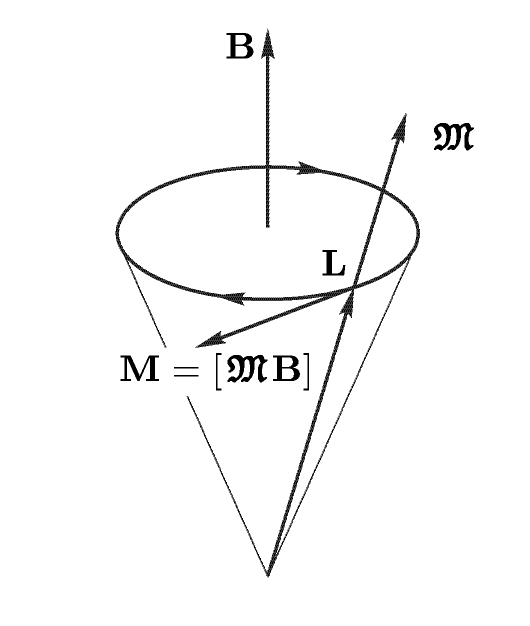
\includegraphics[width=0.4\textwidth]{conus.png}
    \caption{Конус}
    \label{fig:176}
  \end{wrapfigure}

  \begin{equation}
    \boldsymbol{\Omega} = -\Gamma\mathbf{B}
  \end{equation}

  Если момент $\mathbf{L}$ создается орбитальным движением электронов, то $\Gamma=-e /(2 m c)$ и, следовательно, $\Omega=e \mathbf{B} /(2 m c)$, т.е. прецессия происходит с ларморовской частотой. Это показывает, что наша классическая модель приводит к правильному результату. Если же момент L спиновый, то $\Gamma=-e /(m c)$ и угловая скорость прецессии будет вдвое больше. В остальных случаях явление становится более сложным, но его разбор можно найти в \cite{sivykhin5}.

  Учтем теперь столкновения. Если атом получает толчок в направлении прецессионного вращения, то соответствующий ему момент сил вызовет прецессию вокруг оси, перпендикулярной к магнитному полю. С помощью уравнения моментов нетрудно убедиться, что в результате такого толчка угол между векторами $\mathfrak{M}$ и В увеличится. Если же толчок произведен в направлении, противоположном прецессионному вращению, то этот угол уменьшится. Толчки первого тина размагничивают, а второго - намагничивают парамагнетик. Однако эффект намагничивания будет преобладать над эффектом размагничивания, так как толчки против прецессионного вращения в среднем сильнее толчков противоположного направления, подобно тому как сила сопротивления, испытываемая человеком, будет больше, когда он бежит против ветра, а не по ветру. Мы видим, что магнитное поле только поддерживает, а не создает намагничивание парамагнетика. Намагничивание создается и устанавливается в результате столкновений атомов между собой.

  9. Некоторые металлы, например щелочные, обладают парамагнетизмом, но не подчиняются закону Кюри. Магнитная восприимчивость таких металлов в широких пределах не зависит от температуры. Объяснение этого факта было дано Паули (1900-1958) в 1927 г. Он предположил, что парамагнетизм в этих случаях обусловлен не магнитными моментами ионов кристаллической решетки, а спиновыми магнитными моментами электронов проводимости. Рассматривая эти электроны как газ, подчиняющийся статистике Ферми-Дирака (см. \cite{sivykhin2}), Паули рассчитал его магнитную восприимчивость. Этот расчет приведен в \cite[\S99]{sivykhin3}. Здесь же заметим, что независимость магнитной восприимчивости электронного газа в металлах от температуры является следствием теоремы Нернста. Действительно, при обычных температурах электронный газ в металлах находится в состоянии вырождения. Это означает, что для него такие температуры следует считать близкими к абсолютному нулю и можно воспользоваться теоремой Нернста. Из формулы \ref{eq:term4} следует

  \begin{equation}
  \frac{1}{4 \pi}\left(\frac{\partial B}{\partial T}\right)_H=\left(\frac{\partial S}{\partial H}\right)_T
  \end{equation}

  Правая часть этого соотношения обращается в нуль в силу теоремы Нернста, а левая равна $(H / 4 \pi) d \mu / d T$. Здесь символ $H$ в производной $\partial \mu / \partial T$ опущен, а сама производная написана в виде $d \mu / d T$, так как $\mu$ от $H$ не зависит. Таким образом, $d \mu / d t=4 \pi d \varkappa / d T=0$.

  \section{Заключение}

  \bibliography{references}
  \bibliographystyle{gost}

\end{document}
